\documentclass[a4paper, 11pt]{article}

% パッケージ設定
\usepackage{luatexja}
\usepackage{luatexja-fontspec}
\usepackage[top=25mm, bottom=25mm, left=25mm, right=25mm]{geometry}
\usepackage{graphicx}
\usepackage{listings}
\usepackage{xcolor}
\usepackage{caption}
\usepackage{subcaption}
\usepackage{titlesec}
\usepackage{hyperref}

% 日本語フォント設定

% セクションのタイトルスタイル
\titleformat{\subsection}{\large\bfseries}{\thesubsection}{1em}{}
\titleformat{\subsubsection}{\normalsize\bfseries}{\thesubsubsection}{1em}{}

% コード表示のスタイル
\lstset{
basicstyle=\ttfamily\footnotesize,
backgroundcolor=\color{gray!10},
frame=single,
numbers=left,
numberstyle=\tiny,
breaklines=true,
captionpos=b
}

% ハイパーリンク設定
\hypersetup{
colorlinks=true,
linkcolor=blue,
urlcolor=cyan
}

% タイトル
\title{コンピュータアーキテクチャ最終レポート}
\author{杉山月渚(03-230426)}
\date{\today}

\begin{document}

\maketitle

\section{課題1}
「プロセッサをHDLで書いてみよう – シングルサイクル・プロセッサでOK」について以下にまとめる。
単一サイクル構成のRISC-Vプロセッサの実装における各Verilogファイルの役割と、その動作を示す波形画像について解説する。

\subsection{回路構成と各モジュールの役割}
本プロセッサは以下のコンポーネントから構成されている~\cite{sakai2004computer_architecture}:

\subsubsection{\texttt{riscv\_single\_cycle.v}}
CPU全体のトップモジュールであり、各コンポーネントを接続する役割を果たす。
クロックとリセットを入力とし、プログラムカウンタ、命令メモリ、レジスタファイル、ALU、制御ユニットなどを結合する。

\lstinputlisting[language=Verilog, caption=CPUトップモジュール, label=lst:singlecycle]{q1_riscv/riscv_single_cycle.v}

\subsubsection{\texttt{pc\_unit.v}}
プログラムカウンタ(PC)を保持し、分岐やジャンプ命令に応じて次の命令アドレスを供給する。

\lstinputlisting[language=Verilog, caption=PC管理ユニット, label=lst:pc]{q1_riscv/pc_unit.v}

\subsubsection{\texttt{instruction\_memory.v}}
命令ROMとして動作し、プログラムカウンタから指定された命令を返す。
\texttt{mem}配列にテスト用命令が事前に格納されている。

\lstinputlisting[language=Verilog, caption=命令メモリ, label=lst:imem]{q1_riscv/instruction_memory.v}

\subsubsection{\texttt{register\_file.v}}
32本のレジスタを持ち、読み出し・書き込み操作を制御信号に基づいて実行する。
デバッグ用にx0〜x6の出力も提供している。

\lstinputlisting[language=Verilog, caption=レジスタファイル, label=lst:regfile]{q1_riscv/register_file.v}

\subsubsection{\texttt{alu.v}}
加算・減算・論理演算などを行う演算器。\texttt{alu\_op}信号により動作内容が決定される。

\lstinputlisting[language=Verilog, caption=ALU, label=lst:alu]{q1_riscv/alu.v}

\subsubsection{\texttt{control\_unit.v}}
命令の\texttt{opcode}, \texttt{funct3}, \texttt{funct7}から各種制御信号(レジスタ書き込み許可、ALU操作、分岐、メモリ読み書きなど)を生成する。

\lstinputlisting[language=Verilog, caption=制御ユニット, label=lst:control]{q1_riscv/control_unit.v}

\subsubsection{\texttt{sign\_extender.v}}
I/B/U/J型命令の即値を符号拡張して32ビットに変換するユニット。

\lstinputlisting[language=Verilog, caption=即値生成ユニット, label=lst:sext]{q1_riscv/sign_extender.v}

\subsubsection{\texttt{data\_memory.v}}
ロード(\texttt{lw})・ストア(\texttt{sw})命令に使用されるデータメモリ。
読み書きは\texttt{mem\_read\_en}と\texttt{mem\_write\_en}により制御される。

\lstinputlisting[language=Verilog, caption=データメモリ, label=lst:dmem]{q1_riscv/data_memory.v}

\subsection{動作波形と確認}
以下に、ALU演算やジャンプ命令の動作確認を行ったときの波形を示す。

\subsubsection{add, sub, xor命令}
\begin{lstlisting}
    // I-type
    mem[0]  = 32'b000000000001_00000_000_00001_0010011; // addi x1, x0, 1     → x1 = 1
    mem[1]  = 32'b000000000010_00000_000_00010_0010011; // addi x2, x0, 2     → x2 = 2

    // R-type
    mem[2]  = 32'b0000000_00010_00001_000_00011_0110011; // add x3, x1, x2    → x3 = x1 + x2 = 3
    mem[3]  = 32'b0100000_00001_00011_000_00100_0110011; // sub x4, x3, x1    → x4 = x3 - x1 = 2
\end{lstlisting}

\begin{figure}[h]
\centering
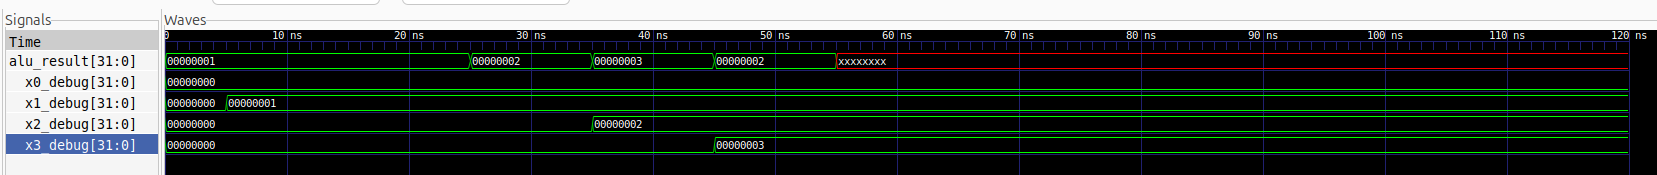
\includegraphics[width=0.8\textwidth]{images/add.png}
\caption{I, R-type命令の動作波形}
\label{fig:addwave}
\end{figure}

\subsubsection{or, and, sll, srl命令}
\begin{lstlisting}
    // I-type
    mem[0]  = 32'b000000000001_00000_000_00001_0010011; // addi x1, x0, 1     → x1 = 1
    mem[1]  = 32'b000000000010_00000_000_00010_0010011; // addi x2, x0, 2     → x2 = 2

    // R-type
    mem[2]  = 32'b0000000_00010_00001_000_00011_0110011; // add x3, x1, x2    → x3 = x1 + x2 = 3
    mem[3]  = 32'b0100000_00001_00011_000_00100_0110011; // sub x4, x3, x1    → x4 = x3 - x1 = 2
    mem[4]  = 32'b0000000_00010_00011_100_00101_0110011; // xor x5, x3, x2    → x5 = x3 ^ x2 = 1
    mem[5]  = 32'b0000000_00010_00011_110_00110_0110011; // or  x6, x3, x2    → x6 = x3 | x2 = 3
    mem[6]  = 32'b0000000_00010_00011_111_00111_0110011; // and x7, x3, x2    → x7 = x3 & x2 = 2
    mem[7]  = 32'b0000000_00010_00011_001_01000_0110011; // sll x8, x3, x2    → x8 = x3 << x2 = 12
    mem[8]  = 32'b0000000_00010_00011_101_01001_0110011; // srl x9, x3, x2    → x9 = x3 >> x2 = 0
\end{lstlisting}

\begin{figure}[h]
\centering
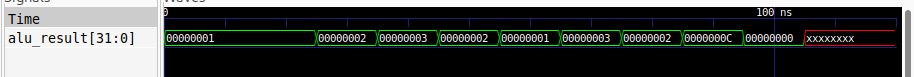
\includegraphics[width=0.8\textwidth]{images/load.png}
\caption{or, and, sll, srl命令の動作波形}
\label{fig:addwave}
\end{figure}

\subsubsection{lw, sw命令}
\begin{lstlisting}
    // I-type
    mem[0]  = 32'b000000000001_00000_000_00001_0010011; // addi x1, x0, 1     → x1 = 1
    mem[1]  = 32'b000000000010_00000_000_00010_0010011; // addi x2, x0, 2     → x2 = 2

    // R-type
    mem[2]  = 32'b0000000_00010_00001_000_00011_0110011; // add x3, x1, x2    → x3 = x1 + x2 = 3
    mem[3]  = 32'b0100000_00001_00011_000_00100_0110011; // sub x4, x3, x1    → x4 = x3 - x1 = 2
    mem[4]  = 32'b0000000_00010_00011_100_00101_0110011; // xor x5, x3, x2    → x5 = x3 ^ x2 = 1
    mem[5]  = 32'b0000000_00010_00011_110_00110_0110011; // or  x6, x3, x2    → x6 = x3 | x2 = 3
    mem[6]  = 32'b0000000_00010_00011_111_00111_0110011; // and x7, x3, x2    → x7 = x3 & x2 = 2
    mem[7]  = 32'b0000000_00010_00011_001_01000_0110011; // sll x8, x3, x2    → x8 = x3 << x2 = 12
    mem[8]  = 32'b000000000000_00010_111_00101_0000011;  // lw   x5, 0(x8)      → x5 = MEM[x8+0]
\end{lstlisting}

\begin{figure}[h]
\centering
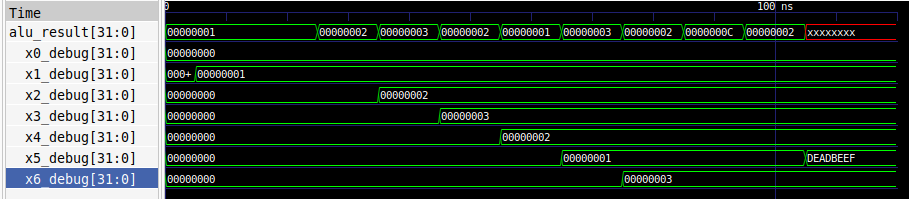
\includegraphics[width=0.8\textwidth]{images/lw.png}
\caption{or, and, sll, srl命令の動作波形}
\label{fig:addwave}
\end{figure}

\subsubsection{beq, bne命令}
\begin{lstlisting}
    // I-type
    mem[0]  = 32'b000000000001_00000_000_00001_0010011; // addi x1, x0, 1     → x1 = 1
    mem[1]  = 32'b000000000010_00000_000_00010_0010011; // addi x2, x0, 2     → x2 = 2

    // R-type
    mem[2]  = 32'b0000000_00010_00001_000_00011_0110011; // add x3, x1, x2    → x3 = x1 + x2 = 3
    mem[3]  = 32'b0100000_00001_00011_000_00100_0110011; // sub x4, x3, x1    → x4 = x3 - x1 = 2
    mem[4]  = 32'b0000000_00010_00011_100_00101_0110011; // xor x5, x3, x2    → x5 = x3 ^ x2 = 1

    // B-type
    mem[5] = 32'b0000000_00011_00010_000_01000_1100011; // beq x2, x3, +8    → branch not taken
    mem[6] = 32'b0000000_00011_00010_001_01000_1100011; // bne x2, x3, +8    → branch taken

    // U-type
    mem[7] = 32'b00000000000000000001_00101_0110111;   // lui x5, 0x0       → x5 = 0x00000000
    mem[8] = 32'b00010010001101000101_00001_0110111;   // lui x1, 0x12345  → x13 = 0x12345000
\end{lstlisting}
\begin{figure}[h]
\centering
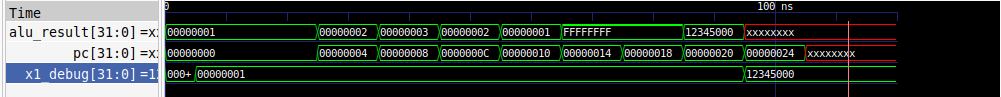
\includegraphics[width=0.8\textwidth]{images/b_u_type.png}
\caption{B-type, U-type命令の動作波形}
\label{fig:addwave}
\end{figure}


\subsubsection{jal命令}
\begin{lstlisting}
    // I-type
    mem[0]  = 32'b000000000001_00000_000_00001_0010011; // addi x1, x0, 1     → x1 = 1
    mem[1]  = 32'b000000000010_00000_000_00010_0010011; // addi x2, x0, 2     → x2 = 2

    // R-type
    mem[2]  = 32'b0000000_00010_00001_000_00011_0110011; // add x3, x1, x2    → x3 = x1 + x2 = 3
    mem[3]  = 32'b0100000_00001_00011_000_00100_0110011; // sub x4, x3, x1    → x4 = x3 - x1 = 2
    mem[4]  = 32'b0000000_00010_00011_100_00101_0110011; // xor x5, x3, x2    → x5 = x3 ^ x2 = 1

    mem[5] = 32'h002000ef;  // jal x1, 4
\end{lstlisting}
\begin{figure}[h]
\centering
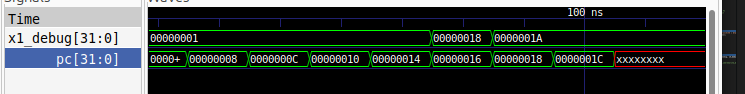
\includegraphics[width=0.8\textwidth]{images/jal.png}
\caption{jal命令の動作波形(x1にPC+4が保存される)}
\label{fig:jalwave}
\end{figure}

\section{課題2}
2023年以降に主要なコンピュータアーキテクチャ会議で発表された論文の中から、「FlashLLM: A Chiplet-Based In-Flash Computing Architecture to Enable On-Device Inference of 70B LLM」(MICRO 2024)\cite{yu2024cambriconllmchipletbasedhybridarchitecture}を選定し、その概要と将来のアーキテクチャ課題への貢献について詳述する。
この論文は、大規模言語モデル(LLM)をスマートフォンや車両などのエッジデバイスに展開する際の、メモリ帯域幅の制約と電力効率の課題に正面から取り組んでいる。
FlashLLMは、チップレット技術を介してNPU(ニューラルプロセッシングユニット)に直接接続された専用のフラッシュチップを特徴とする、革新的なハイブリッドアーキテクチャを提案している。
この設計は、モデルの重みを行動中にフラッシュメモリ内で処理する「インフラッシュコンピューティング」の概念を導入することで、データ転送量を劇的に削減し、結果として推論速度とエネルギー効率を大幅に向上させている。

\subsection{モチベーション: エッジデバイスにおけるLLM展開の課題}
大規模言語モデル(LLM)は、そのテキスト生成能力により、現代の自然言語処理の中核を担っている。
ChatGPTの急速な普及が示すように、LLMはすでにテクノロジー業界の製品に深く組み込まれている。
しかし、LLMは数十億から数兆に及ぶ膨大な数のパラメータを必要とし、スマートフォンや車両などのリソースが限られたエッジデバイスへの展開において、重大な課題を提起している。
既存のフラッシュオフロード技術では、モデルの重みをフラッシュベースのストレージにオフロードする研究が盛んに行われているが、
フラッシュメモリの限られた帯域幅が推論速度を著しく阻害するという問題がある。
特に、エッジ推論シナリオではバッチサイズが1であり、演算強度が最小限であるため、この帯域幅の制約がボトルネックとなる。
これは、プロセッサとメモリ間のデータ転送速度の不均衡を示す「メモリウォール」問題が、LLMの文脈でさらに悪化していることを意味する。

\subsection{アイデア:FlashLLMのチップレットベースハイブリッドアーキテクチャ}
課題に対処するため、FlashLLMは70B LLMのオンデバイス推論のために特別に設計された、チップレットベースのハイブリッドアーキテクチャを導入している。
このアーキテクチャは、以下の主要コンポーネントで構成される:
\begin{itemize}
    \item 専用フラッシュチップ: チップレット技術を介してニューラルプロセッシングユニット(NPU)に直接接続されている。主な目的は、モデルの重み行列を保存することと、オンダイ処理能力を活用してデータ転送を削減することである
    \item ニューラルプロセッシングユニット(NPU): フラッシュチップと連携して行列演算を実行する。さらに、NPUはDRAM内のキーバリュー(KV)キャッシュを管理し、フラッシュのオンダイ処理能力を超える特殊な機能計算を担当する。
\end{itemize}

\subsection{効果}
\begin{table}[h]
  \centering
  \caption{LLMモデルにおける推論速度と高速化率~\cite{yu2024cambriconllmchipletbasedhybridarchitecture}}
  \begin{tabular}{|c|c|c|}
    \hline
    \textbf{LLMモデルサイズ} & \textbf{推論速度(トークン/秒)} & \textbf{既存のフラッシュオフロード技術に対する速度向上} \\
    \hline
    70B & 3.44  & 22倍以上 \\
    7B  & 36.34 & 45倍以上 \\
    \hline
  \end{tabular}
  \label{tab:llm_speedup}
\end{table}
Table~\ref{tab:llm_speedup}が示すように、FlashLLMは、70B LLMで3.44トークン/秒、7B LLMで36.34トークン/秒の推論速度を達成し、既存のフラッシュオフロード技術と比較して22倍から45倍の速度向上を実現している。
この性能向上は、メモリ帯域幅、容量、電力という複数のボトルネックに同時に取り組む、多層的な解決策の有効性を示している。

\subsection{将来のアーキテクチャ課題への貢献}
FlashLLMが示す方向性は、将来的な「オンデバイスLLM」における以下の課題に答えている:
\begin{itemize}
    \item 帯域制約と電力消費の克服:データを「動かす」より「現地で計算する」アプローチ
    \item チップレット技術の実用化:SoC外部の非DRAM記憶装置との協調演算という新しいデザイン空間
    \item 誤り訂正との統合アーキテクチャ:誤りに脆弱なフラッシュでもAI推論が実行可能になる設計の第一歩
\end{itemize}

\bibliographystyle{plain}
\bibliography{references} % if you use a .bib file
\end{document}

